The main idea of the inverse function theorem is that given a suitably ``nice'' mapping, one might be able to determine whether or not an inverse mapping exists and it might possibly have some nice properties. To motivate the statements that our theorems have we will explore some examples in the one dimensional case. First, we might recall that if $f'(x) > 0$ on some interval $[a, b]$ this implies that $f$ is increasing on $[a, b]$. Let's consider a related question: Suppose we know at some point $x$ that $f'(x) = 0$. Does that mean there is some interval containing $x$ where $f$ is increasing? The answer is no. To see this, we might consider the graph of the function $f(x) = x^2\sin(1/x)$:

\begin{figure}[h]
	\centering
	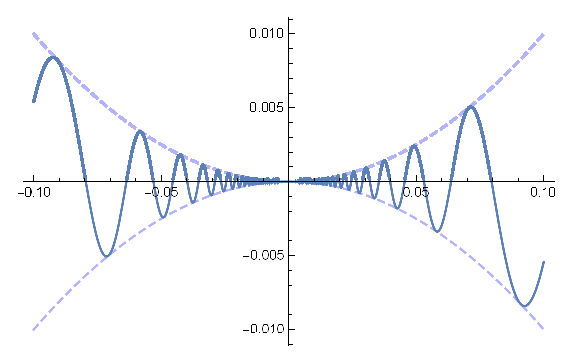
\includegraphics{plots_gr1.eps}
	\caption{The graph of $f(x) = x^2\sin(1/x)$}
	\label{fig:plots_gr1}
\end{figure}

It is straightforward to see that $f$ is differentiable everywhere but $0$, and if we further define $f$ so that $f(0) = 0$, we see that $f(x)$ is differentiable at $0$ with $f'(0) = 0$.

Similarly, we can consider the function 
\[f(x) = \begin{cases} 0 & x = 0 \\ \frac{x}{2} + x^2\sin(1/x) & \text{otherwise.} \end{cases}\]
Then $f'(0) = 1/2$. However, it is straightforward to show that $f(x)$ is not increasing on any interval containing $f(0) = 0$. That is, there are points as close to $0$ as we would like where the derivative is less than $0$.

\begin{figure}[h]
	\centering
	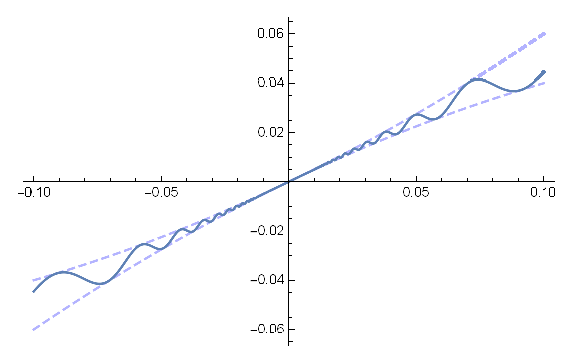
\includegraphics{plots_gr2.eps}
	\caption{The graph of $f(x) = \frac{x}{2} + x^2\sin(1/x)$}
	\label{fig:plots_gr2}
\end{figure}

So simply the derivative being non-zero at a point does not give us an interval containing that point where the function $f$ is increasing. In particular, there is no interval around that point where $f$ is \textit{invertible} when restricted to that interval. So what went wrong here? Let's take the derivative of $x^2\sin(1/x)$ when $x \neq 0$:
\[\frac{d}{dx}(x^2\sin(1/x)) = 2x\sin(1/x) - \cos(1/x).\]
Notice that this function does not have a limit at $0$. It follows that $f'$ is \textbf{not} continuous at $0$, even though it is defined there. It will turn out that the sufficient condition necessary is that the derivative at a point $x$ is non-zero and $f'$ is both non-zero and continuous at $x$, that is continuously differentiable ($\CD{1}$).

Here is the theorem we will prove (the Inverse Function Theorem):

\begin{theorem}
Suppose $U$ is an open subset in $\Real^n$, and $f: U \to \Real^n$ is a $\CD{1}$ function. Suppose $a \in U$ and $Df(a): \Real^n \to \Real^n$ is an invertible linear mapping. Then there is some neighborhood $V$ of $a$, where $V \subset U$, such that 
\begin{itemize}
	\item $f$ is injective on $V$
	\item $f|_V$ is an open mapping,
	\item There exists a $\CD{1}$ function $g: f(V) \to V$ which is an inverse of $f$.
\end{itemize}
Moreover, for any $y = f(x) \in W$,
\[Dg(y) = Df(x)^{-1}.\]
\end{theorem}

In fact, the easiest thing to prove is the last statement. For all $x \in V$ we have that 
\[g(f(x)) = x \implies Dg(f(x))Df(x) = I,\] by the chain rule. Composition of the inverse $Df(x)^{-1}$ gives us the desired formula.